\begin{frame}
    \titlepage
\end{frame}

{
\setbeamercolor{background canvas}{bg=blue!40!black,fg=blue!10!white}
\setbeamercolor{normal text}{bg=blue!40!black,fg=blue!10!white}
\setbeamercolor{itemize/enumerate body}{fg=white}
\setbeamercolor{itemize/enumerate subbody}{fg=white}
\setbeamercolor{titlelike}{bg=blue!40!black,fg=blue!10!white}
\begin{frame}<1|handout:1>[noframenumbering]{Changelog}
    \begin{itemize}
        \item Corrections made in this version not in first posting:
        \begin{itemize}
            \item 3 April 2017: Fix ROP with VTable overwrite example (slide 11) to
            use \%rsi instead of \%rdi. I somehow thought *(\%rdi) was
            looking for a pointer to pointer when it certainly does not
        \end{itemize}
    \end{itemize}
\end{frame}
}

\tikzset{
    stackBox/.style={very thick},
    allocBox/.style={dashed,very thick,fill=blue!20},
    onStack/.style={thick},
    frameOne/.style={fill=blue!15},
    frameTwo/.style={fill=red!15},
    markLine/.style={blue!50!black},
    markLineB/.style={red!90!black},
    hiLine/.style={red!90!black},
}

\begin{frame}{last time}
    \begin{itemize}
        \item ASLR --- random addresses
            \begin{itemize}
            \item performance/compatibility concerns
            \end{itemize}
        \item write XOR execute --- no injecting machine code
            \begin{itemize}
            \item minor compatibility concerns
            \end{itemize}
        \item ROP --- defeating write XOR execute
    \end{itemize}
\end{frame}

\begin{frame}{logistical notes}
    \begin{itemize}
        \item exam review --- questions?
        \item FORMAT
        \item on the final
            \begin{itemize}
            \item likely part take-home, part in-class
            \end{itemize}
    \end{itemize}
\end{frame}

\begin{frame}[fragile,label=loadChain]{ROP chain}
\begin{tikzpicture}
% FIXME:
\tikzset{
    stackBox/.style={very thick},
    onStack/.style={thick},
    useLine/.style={very thick,blue,Latex-},
    useLineRet/.style={red,very thick,-Latex,dashed},
    gadgetBox/.style={blue,thick,text=black,draw,align=left,font=\small},
}
\begin{scope}[xscale=0.75]
\draw[stackBox] (0, 3) rectangle (10, -3);
\draw[thick,-Latex] (-.25,-1) -- (-.25, 1) node [midway, above, sloped] {increasing addresses};
\draw[onStack,fill=green!20,opacity=0.9] (0, 3.00) rectangle (10, 1.75) node[midway,align=center,font=\small] (theString)
     {string to print};
\draw[onStack,red] (0, 1.75) rectangle (10, .75) node[midway,align=center,font=\small] (gadgetTwo)
     {pointer to second gadget};
\draw[onStack,fill=green!20] (0, .75) rectangle (10, -.25) node[midway,align=center,font=\small] (putsAddr)
     {address of \texttt{puts} (popped from stack)};
\draw[onStack,red] (0, -.25) rectangle (10, -1.25) node[midway,align=center,font=\small] (stackAddr)
     {return address for {\tt vulnerable}: \\pointer to first gadget};
\draw[onStack,fill=blue!20] (0, -1.25) rectangle (10, -2.25) node[midway,align=center,font=\small] {buffer (100 bytes)};
\draw[onStack,fill=red!20,opacity=0.9] (0, -2.25) rectangle (10, -1.25) node[midway,align=center,font=\small,text=red!50!black] {unused junk};
        \draw[-Latex,red,ultra thick,dashed] (stackAddr.east) -- ++(3cm,0cm) 
        node[right,gadgetBox] (firstGad) { {\tt popq \%rax} \\ {\tt ret} };
        \draw[-Latex,red,ultra thick,dashed] (gadgetTwo.east) -- ++(3cm,0cm)
        node[right,gadgetBox] (secondGad) { {\tt mov \%rsp, \%rdi} \\ {\tt call *\%rax} };
    \begin{visibleenv}<2->
        \node[gadgetBox,dashed,below=1cm of firstGad] (realRet) {
            \texttt{ret} (in vulnerable)
        };
        \draw[useLineRet] ([xshift=1ex]realRet.west) -- ([xshift=-1ex,yshift=2ex]stackAddr.south east);
    \end{visibleenv}
    \begin{visibleenv}<3->
        \draw[useLine] ([yshift=.6em,xshift=1ex]firstGad.west) -- (putsAddr.east);
    \end{visibleenv}
    \begin{visibleenv}<4->
        \draw[useLineRet] ([yshift=-.6em,xshift=1ex]firstGad.west) -- ([xshift=-1ex,yshift=2ex]gadgetTwo.south east);
    \end{visibleenv}
    \begin{visibleenv}<4->
        \draw[useLine] ([yshift=.6em,xshift=1ex]secondGad.west) -- (theString.east);
    \end{visibleenv}
\end{scope}
\end{tikzpicture}
\end{frame}

\begin{frame}{gadgets generally}
    \begin{itemize}
        \item bits of machine code that do work, then return or jump
        \item ``chain'' together, by having them jump to each other
        \item most common: find gadget ending with \texttt{ret}
            \begin{itemize}
            \item pops address of next gadget offs tack
            \end{itemize}
        \item can do pretty much anything
    \end{itemize}
\end{frame}

\begin{frame}{ROP and ASLR}
    \begin{itemize}
    \item find a pointer to known thing in libc (or other source of gadgets)
        \begin{itemize}
        \item e.g. information leak from use-after-free
        \end{itemize}
    \item use that to compute address of all gadgets
    \item then address randomization doesn't matter
    \end{itemize}
\end{frame}

\begin{frame}{ROP and write XOR execute}
    \begin{itemize}
    \item all the code we're running is supposed to be executed
    \item completely defeats write XOR execute
    \end{itemize}
\end{frame}

\begin{frame}{ROP and stack canaries}
    \begin{itemize}
    \item information disclosure reveals canary value if needed, still
    \item full stack canaries should reduce number of gadgets
        \begin{itemize}
        \item no real returns without canary checks
        \end{itemize}
    \item \ldots but typically only canaries if stack-allocated buffer
    \item and return opcodes within other instructions
    \end{itemize}
\end{frame}

\begin{frame}{ROP without a stack overflow (1)}
    \begin{itemize}
    \item e.g. VTable overwrite
    \item look for gadget(s) that set {\tt \%rsp}
    \item \ldots based on function argument registers/etc.
    \end{itemize}
\end{frame}

\begin{frame}{ROP without stack overflow (2)}
    \begin{itemize}
    \item example sequence:
        \begin{itemize}
            \item \sout{\texttt{push \%rdi; call *(\%rdx)}}
                \begin{itemize}
                    \item forgot to account for call last time
                \end{itemize}
            \item \texttt{push \%rdx; jmp *(\%rsi)}
            \item \texttt{pop \%rsp; ret}
        \end{itemize}
    \item set:
        \begin{itemize}
        \item overwritten vtable entry = pointer to first gadget
        \item arg 2: {\tt \%rsi} = pointer to pointer to second gadget
        \item arg 3: {\tt \%rdx} = desired stack pointer
        \end{itemize}
    \end{itemize}
\end{frame}

\begin{frame}[fragile,label=VTblOver]{VTable overwrite with gadget}
\lstset{language=C++,style=small}
    \begin{tikzpicture}
        \node[anchor=north east] (code) at (1.5, 0) {
\begin{lstlisting}
class Bar {
  char buffer[100];
  Foo *foo;
  int x, y;
  ...
};

void Bar::vulnerable() {
  gets(buffer);
  foo->some_method(x, y);
  // (*foo->vtable[K])(foo, x, y)
  // foo == rdi, x == rsi, y == rdx
}
\end{lstlisting}
};
\tikzset{
    stackBox/.style={very thick},
    onStack/.style={thick},
    useLine/.style={very thick,blue,Latex-},
    useLineRet/.style={red,very thick,-Latex,dashed},
    gadgetBox/.style={blue,thick,text=black,draw,align=left,font=\small},
}
        \begin{visibleenv}<1-2>
\draw[thick,-Latex] (-.25,-4) -- (-.25, -1) node [midway, above, sloped] {increasing addresses};
        \end{visibleenv}
    \draw[stackBox] (0, 0) rectangle (3, -5);
        \draw[onStack,fill=green!20] (0, -1.5) rectangle (3, -5) node[midway] {buffer};
        \draw[onStack,fill=yellow!20] (0, -1) rectangle (3, -1.5) node[midway] {foo};
        \draw[onStack,fill=yellow!20] (0, -0) rectangle (3, -1) node[midway] {x, y};

        \draw[stackBox] (4, 0) rectangle (7, -3);
        \draw[onStack](4, -2.5) rectangle (7, -3) node[midway] {vtable ptr};

        \draw[stackBox] (4, -4) rectangle (7, -6);
        \node[midway,anchor=south] at (5.5, -5) {func. ptrs};
        \draw[fill=blue!30] (4, -5) rectangle (7, -5.5) node[midway] { some\_method };

        \draw[-Latex, very thick,blue] (3, -1.25) -- ++ (.5cm, 0) |- (4, -2.9);
        \draw[-Latex, very thick,blue] (7, -2.75) -- ++ (.5cm, 0) |- (7, -5.9);
        \begin{visibleenv}<2->
            \fill[pattern=north west lines,pattern color=red] (0, -0) rectangle (3, -1.5);
            \draw[-Latex, ultra thick, dashed, red] (3, -1.25) -- ++(.5cm, 0) |- (3, -4.9);
            \draw[fill=white,fill opacity=0.9,draw=red,very thick] (0, -5) rectangle (3, -4.5)
                node[midway] {``vtable'' ptr};
        \end{visibleenv}
        \begin{visibleenv}<3->
            \draw[fill=blue!30,fill opacity=0.9,draw=red,very thick] (0, -2.5) rectangle (3, -2)
                node[midway] {\text{gadget} ptr};
            \draw[-Latex, ultra thick, dashed, red] (0, -4.75) -- ++(-.5cm, 0) |- (0, -3);
            \draw[fill=white,fill opacity=0.9,draw=red,very thick] (0, 0) rectangle (3, -1)
                node[midway] { \textbf{rsi}, \textbf{rdx} values };
            \draw[Latex-, thick,red] (3, -5) -- ++(0cm, -.5cm) node[below] {rdi value};
        \end{visibleenv}
        \begin{visibleenv}<4->
            \node[align=left,thick,draw,anchor=north east,fill=white] (gadget) at (-1, -3) {
                gadget: \\ \texttt{push \%rdx; jmp *(\%rsi)}
            };
            \draw[-Latex,ultra thick, dashed, red] (0, -2.25) -| (gadget.north);
        \end{visibleenv}
    \end{tikzpicture}
\end{frame}



\begin{frame}{jump-oriented programming}
    \begin{itemize}
        \item just look for gadgets that end in \texttt{call} or \texttt{jmp}
        \item don't even need to set stack
        \item harder to find than \texttt{ret}-based gadgets
            \begin{itemize}
            \item but almost always as powerful as ret-based gadgets
            \end{itemize}
        \item makes return-oriented programming mitigation hard
            \begin{itemize}
            \item can't just protect all \texttt{ret}s (in middle of instruction or not)
            \end{itemize}
    \end{itemize}
\end{frame}

\begin{frame}{finding gadgets}
    \begin{itemize}
        \item find code segments of exectuable/library
        \item look for opcodes of arbitrary jumps:
            \begin{itemize}
            \item \texttt{ret}
            \item \texttt{jmp *register}
            \item \texttt{jmp *(register)}
            \item \texttt{call *register}
            \item \texttt{call *(register)}
        \end{itemize}
        \item disassemble starting a few bytes before
            \begin{itemize}
            \item invalid instruction? jump before ret? etc. --- discard
            \end{itemize}
        \item sort list
        \vspace{.5cm}
    \item \myemph{automatable}
    \end{itemize}
\end{frame}

\begin{frame}{programming with gadgets}
    \begin{itemize}
        \item can usually find gadgets to:
            \begin{itemize}
            \item pop from stack into argument register
            \item write register to memory location in another register
            \item clear a register
            \end{itemize}
        \item along with gadget for \texttt{syscall} (make OS call) --- can do anything
    \end{itemize}
\end{frame}

\begin{frame}{common, reusable ROP sequences}
    \begin{itemize}
        \item open a command-line --- what \texttt{ROPgadget} tool defaults to 
        \item make memory executable + jump
            \begin{itemize}
            \item generally: just do enough to ignore write XOR execute
            \end{itemize}
        \item often only depend on memory locations in shared library
            \begin{itemize}
            \item works across programs --- e.g. many programs use the C standard library
            \end{itemize}
    \end{itemize}
\end{frame}

\begin{frame}{ROP ideas}
    \begin{itemize}
        \item incidental \textit{existing} snippets of code
    \item chain together with non-constant jumps
        \begin{itemize}
        \item returns, function pointer calls, computed jumps
        \end{itemize}
    \item snippets form ``language''
        \begin{itemize}
        \item usually Turing-complete
        \end{itemize}
    \end{itemize}
\end{frame}

\section{Safe C}

\begin{frame}{next topic: fixing real problems}
    \begin{itemize}
    \item we've focused on ``band-aid'' solutions
        \begin{itemize}
        \item detect memory corruption; then hope you can do something
        \end{itemize}
    \item first idea everyone has: just add bounds-checking!
        \begin{itemize}
        \item Java, Python do it\ldots
        \end{itemize}
    \end{itemize}
\end{frame}

\begin{frame}[fragile,label=fortifyMemCpyIntro]{adding bounds checking}
\lstset{language=C,style=small}
\begin{lstlisting}
char buffer[42];
memcpy(buffer, attacker_controlled, len);
\end{lstlisting}
    \begin{itemize}
        \item couldn't compiler add check for \texttt{len}
        \item modern Linux: it does
    \end{itemize}
\end{frame}

\begin{frame}[fragile,label=boundsChecking]{added bounds checking}
\lstset{language=C,style=small}
\begin{lstlisting}
char buffer[42];
memcpy(buffer, attacker_controlled, len);
\end{lstlisting}
\lstset{language=myasm,style=small}
\begin{lstlisting}
    subq   $72, %rsp
    leaq   4(%rsp), %rdi
    movslq len, %rdx
    movq   attacker_controlled, %rsi
    movl   $42, %ecx
    call   __memcpy_chk
\end{lstlisting}
    \begin{itemize}
        \item length \texttt{42} passed to \texttt{\_\_memcpy\_chk}
    \end{itemize}
\end{frame}

\begin{frame}{\_FORTIFY\_SOURCE}
    \begin{itemize}
        \item Linux C standard library + GCC features
        \item adds automatic checking to a bunch of string/array functions
        \item even printf (disable \texttt{\%n} unless format string is a constant)
        \vspace{.5cm}
        \item often enabled by default
        \item GCC options:
            \begin{itemize}
                \item \texttt{-D\_FORTIFY\_SOURCE=1} --- enable (backwards-compatible only)
                \item \texttt{-D\_FORTIFY\_SOURCE=2} --- enable (full)
                \item \texttt{-U\_FORTIFY\_SOURCE} --- disable
            \end{itemize}
    \end{itemize}
\end{frame}

\section{Bounds-checking C standard library}

\begin{frame}[fragile,label=nonChecking]{non-checking library functions}
\lstset{language=C,style=small}
    \begin{itemize}
    \item some C library functions make bounds checking hard: 
\begin{lstlisting}
strcpy(destination, source);
strcat(destination, source);
sprintf(destination, format, ...);
\end{lstlisting}
    \item bounds-checking versions (\myemph{added to library later}):
\begin{lstlisting}
/* might not add \0 (!) */
strncpy(destination, source, size);
// destination[size - 1] = '\0';
/* will add \0: */
strncat(destination, source, size);
snprintf(destination, size, format, ...);
\end{lstlisting}
    \end{itemize}
\end{frame}

\begin{frame}[fragile,label=cppBounds]{C++ bounds checking}
\lstset{language=C,style=small}
\begin{lstlisting}
#include <vector>
...
std::vector<int> data;
data.resize(50);
// undefined behavior:
data[60] = 0;
// throws std::out_of_range exception
data.at(60) = 0;
\end{lstlisting}
\end{frame}

\section{Language-level solutions}

\begin{frame}{language-level solutions}
    \begin{itemize}
    \item languages like Python don't have this problem
    \item couldn't we do the same thing in C?
    \end{itemize}
\end{frame}

\subsection{Extending pointers}

\begin{frame}{bounds-checking C}
    \begin{itemize}
    \item there have been many proposals to add bounds-checking to C
    \item including implementations
    \item brainstorm: \myemph{why hasn't this happened?}
    \end{itemize}
\end{frame}

\begin{frame}[fragile,label=addBounds]{easy bounds-checking}
    \lstset{language=C,style=smaller}
\begin{lstlisting}
void vulnerable() {
    char buffer[100];
    int c;
    int i = 0;
    while ((c = getchar()) != EOF && c != '\n') {
        buffer[i] = c;
    }
}
void vulnerable_checked() {
    char buffer[100];
    int c;
    int i = 0;
    while ((c = getchar()) != EOF && c != '\n') {
        CHECK(i >= 100 || i < 0);
        buffer[i] = c;
    }
}
\end{lstlisting}
\end{frame}

\begin{frame}[fragile,label=wrappedPointers]{adding bounds-checking --- fat pointers}
\lstset{
    language=C,
    style=small
}
\begin{lstlisting}
struct MyPtr {
    char *pointer;
    char *minimum;
    char *maximum;
};
\end{lstlisting}
\end{frame}

\begin{frame}[fragile,label=wrappedPtrStrcpy]{adding bounds checking --- strcpy}
\lstset{
    language=C,
    style=small
}
\begin{lstlisting}
MyPtr strcpy(MyPtr dest, const MyPtr src) {
    int i;
    do {
        CHECK(src.pointer + i <= src.maximum);
        CHECK(src.pointer + i >= src.minimum);
        CHECK(dest.pointer + i <= dest.maximum);
        CHECK(dest.pointer + i >= dest.minimum);
        src.pointer[i] = dest.pointer[i];
        i += 1;
        CHECK(src.pointer + i <= src.maximum);
        CHECK(src.pointer + i >= src.minimum);
    } while (src.pointer[i] != '\0');
    return dest;
}
\end{lstlisting}
\end{frame}

\begin{frame}{speed of bounds checking}
    \begin{itemize}
    \item two comparisons for every pointer access?
    \item three times as much space for every pointer?
    \end{itemize}
\end{frame}

\begin{frame}{research example (2009)}
    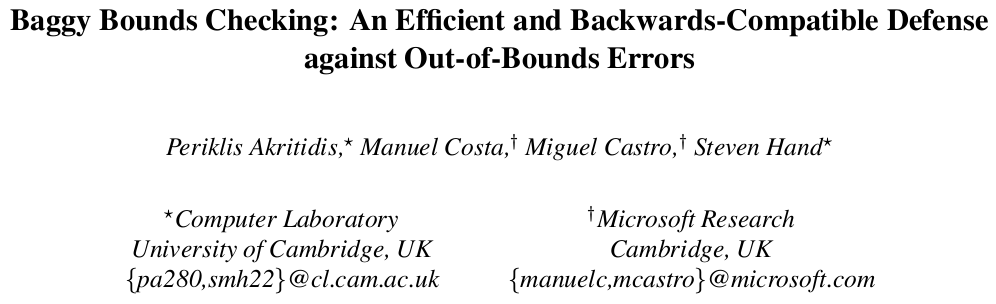
\includegraphics[width=\textwidth]{baggy-bounds-title}
\end{frame}

\begin{frame}[fragile,label=lookupTable]{baggy bounds checking idea}
    \begin{itemize}
        \item giant lookup table --- one entry for every 16 bytes of memory
        \item table indicates start of object allocated here
        \item check pointer arithmetic:
    \end{itemize}
\begin{lstlisting}
char p = str[i];
/* becomes: */
CHECK(START_OF[str / 16] == START_OF[&str[i] / 16]);
char p = str[i];
\end{lstlisting}
\end{frame}


\begin{frame}[fragile,label=baggyBoundsTrick]{baggy bounds trick}
\lstset{language=C,style=small}
    \begin{itemize}
        \item table of pointers to starting locations would be huge
        \item add some restrictions:
            \begin{itemize}
            \item all object sizes are powers of two
            \item all object starting addresses are a multiple of their size
            \end{itemize}
        \item then, table contains size info only:
            \begin{itemize}
            \item table contains $i$, size is $2^i$ bytes:
            \end{itemize}
    \end{itemize}
\begin{lstlisting}
char *GetStartOfObject(char *pointer) {
    return pointer & ~(1 << TABLE[pointer / 16] - 1);
    /* pointer bitwise-and 2^(table entry) - 1 */
    /* clear lower (table entry) bits  of pointer */
}
\end{lstlisting}
\end{frame}

\begin{frame}<1-6>[fragile,label=lkpTble]{allocations and lookup table}
    \begin{tikzpicture}
        \draw[onStack] (0, 0) rectangle (4, -7);
        \draw[allocBox] (0, 0) rectangle (4, -0.4);
        \draw[stackBox] (0, 0) rectangle (4, -0.5);
        \draw[allocBox] (0, -0.5) rectangle (4, -0.8);
        \draw[stackBox] (0, -0.5) rectangle (4, -1.0);
        \draw[allocBox] (0, -1) rectangle (4, -1.9);
        \draw[stackBox] (0, -1) rectangle (4, -2);
        \draw[allocBox] (0, -2) rectangle (4, -2.4);
        \draw[stackBox] (0, -2) rectangle (4, -2.5);
        \draw[allocBox] (0, -2.5) rectangle (4, -2.7);
        \draw[stackBox] (0, -2.5) rectangle (4, -3);
        \draw[stackBox] (0, -3) rectangle (4, -4);
        \draw[allocBox] (0, -4) rectangle (4, -5.2);
        \draw[stackBox] (0, -4) rectangle (4, -6);

        \begin{visibleenv}<1->
            \node[anchor=north west,align=left] at (9, 0) {
                object allocated in \\ \myemph<1>{power-of-two `slots'}
            };
        \end{visibleenv}
        \begin{visibleenv}<2->
            \matrix[tight matrix,
                nodes={text width=1cm,font=\small\tt},anchor=north west,label={north:table}] (tbl) at (7, -1) {
                $2^4$ \\ $2^4$  \\ $2^5$ \\ $2^5$ \\ $2^4$ \\ $2^4$ \\
                $0$ \\ $0$ \\
                $2^6$ \\ $2^6$ \\ $2^6$ \\ $2^6$ \\
            };
            \begin{scope}[thick,dotted,-Latex]
            \draw (4, -.25) -- (tbl-1-1.west);
            \draw (4, -.75) -- (tbl-2-1.west);
            \draw (4, -1.25) -- (tbl-3-1.west);
            \draw (4, -1.75) -- (tbl-4-1.west);
            \draw (4, -2.25) -- (tbl-5-1.west);
            \draw (4, -2.75) -- (tbl-6-1.west);
            \draw (4, -3.25) -- (tbl-7-1.west);
            \draw (4, -3.75) -- (tbl-8-1.west);
            \draw (4, -4.25) -- (tbl-9-1.west);
            \end{scope}
        \end{visibleenv}
        \begin{visibleenv}<3>
            \draw[ultra thick,red] (0, -1) rectangle (4, -2);
            \node[draw,ultra thick,red,inner sep=0mm,fit=(tbl-3-1) (tbl-4-1)] {};
            \draw[ultra thick,blue] (0, -4) rectangle (4, -6);
            \node[draw,ultra thick,blue,inner sep=0mm,fit=(tbl-9-1) (tbl-12-1)] {};
        \end{visibleenv}
        \begin{visibleenv}<3->
            \node[anchor=north west,align=left] at (9, -2) {
                table stores sizes \\
                \myemph{for each 16 bytes}
            };
        \end{visibleenv}
        \begin{visibleenv}<4>
            \draw[ultra thick,red] (0, -3) rectangle (4, -4);
            \node[draw,ultra thick,red,inner sep=0mm,fit=(tbl-7-1) (tbl-8-1)] {};
        \end{visibleenv}
        \begin{visibleenv}<4->
            \node[anchor=north west,align=left] at (9, -3.5) {
                addresses \textbf<4>{multiples of size} \\
                (may \myemph{require padding})
            };
        \end{visibleenv}
        \begin{pgfonlayer}{bg}
        \begin{visibleenv}<5>
            \fill[red!30] (0, -5.2) rectangle (4, -6.);
            \fill[red!30] (0, -2.7) rectangle (4, -3.);
            \fill[red!30] (0, -1.9) rectangle (4, -2.);
            \fill[red!30] (0, -2.4) rectangle (4, -2.5);
            \fill[red!30] (0, -0.8) rectangle (4, -1.);
            \fill[red!30] (0, -0.4) rectangle (4, -0.5);
        \end{visibleenv}
        \end{pgfonlayer}
        \begin{visibleenv}<5->
            \node[anchor=north west,align=left] at (9, -5.5) {
                sizes are \textbf<5>{powers of two} \\
                (may \myemph{require padding})
            };
        \end{visibleenv}
    \end{tikzpicture}
\end{frame}

\begin{frame}[fragile,label=managing]{managing the table}
    \begin{itemize}
        \item not just done \texttt{malloc()/new}
        \item also for stack allocations:
    \end{itemize}
    \begin{lstlisting}[style=small,language=C]
void vulnerable() {
    char buffer[100];
    gets(vulnerable);
}
\end{lstlisting}
    \begin{tikzpicture}[remember picture, overlay]
        \node[anchor=north east] at ([xshift=-.25cm, yshift=-1cm]current page.north east) {
    \begin{lstlisting}[style=small,language=myasm]
vulnerable:
  // make %rsp a multiple
  // of 128 (2^7) 
  andq $0xFFFFFFFFFFFFFF80, %rsp
  // allocate 128 bytes
  subq $0x80, %rsp
  // rax <- rsp / 16
  movq $rsp, %rax
  shrq $4, %rax
  movb $7, TABLE(%rax)
  movb $7, TABLE+1(%rax)
  ...
  movq %rsp, %rdi
  call gets
  ret
\end{lstlisting}
};
    \end{tikzpicture}
\end{frame}

\begin{frame}[fragile,label=sparseLookup]{sparse lookup table}
    \begin{tikzpicture}
        \node[anchor=south] at (3.5, 3) {lookup table};
        \draw[stackBox] (0, 3) rectangle (7, -3);
        \draw[pattern color=red,pattern=north west lines,onStack] (0, -3) rectangle (7, -1.5)
            node[midway,fill=white,align=center] {unallocated memory (segfault) };
        \draw[fill=green,onStack] (0, -1.5) rectangle (7, .2)
            node[midway] { allocated part of table };
        \draw[pattern color=red,pattern=north west lines,onStack] (0, .20) rectangle (7, 1.3)
            node[midway,fill=white,align=center] {unallocated memory (segfault) };
        \draw[fill=green,onStack] (0, 1.3) rectangle (7, 1.6);
        \draw[pattern color=red,pattern=north west lines,onStack] (0, 1.6) rectangle (7, 2.3);
        \draw[fill=green,onStack] (0, 2.3) rectangle (7, 3)
            node[midway] { allocated part of table };
    \end{tikzpicture}
\end{frame}

\begin{frame}{baggy bounds check: added code}
    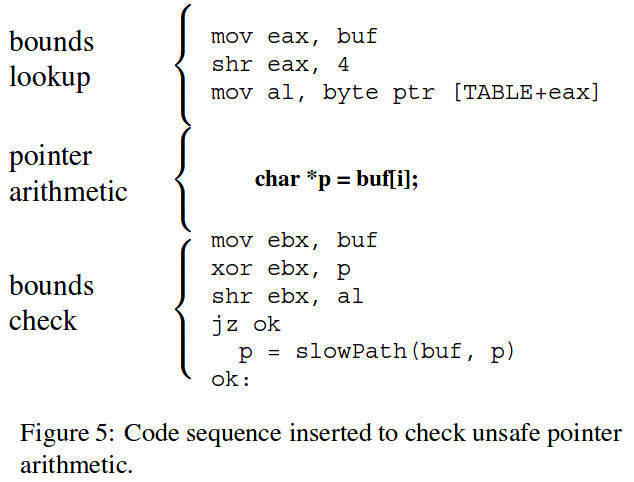
\includegraphics[width=0.6\textwidth]{bb-bounds-check}
\end{frame}

\begin{frame}[fragile,label=addedCode]{baggy bounds check: added code}
    \lstset{language=myasm,style=small}
    \begin{lstlisting}
/* bounds lookup */
    mov buf, %rax
    shr %rax, 4
    mov LOOKUP_TABLE(%rax), %al
/* array element address computation */
    ...    // `\textbf{\textit{char * p = buf[i];}}`
/* bound check */
    mov buf, %rbx
    xor p, %rbx
    shr %al, %rbx
    jz  ok
    ...    // handle possible violation
ok:
\end{lstlisting}

    \imagecredit{adapted from paper figure}
\end{frame}

\begin{frame}{avoiding checks}
    \begin{itemize}
        \item code not added if not array/pointer accesses to object
        \item code not added when pointer accesses ``obviously'' safe
            \begin{itemize}
            \item author's implementation: only checked within function
            \end{itemize}
    \end{itemize}
\end{frame}

\begin{frame}{alternate approach: pointer tagging}
    \begin{itemize}
        \item some bits of \myemph{address} are size 
        \begin{itemize}
        \item replaces table entry/lookup
        \end{itemize}
    \item change code to allocate objects this way
    \item works well on 64-bit --- plenty of addresses to use
    \end{itemize}
    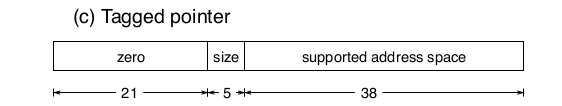
\includegraphics[width=0.8\textwidth]{baggy-bounds-tagging}
\end{frame}

\begin{frame}{baggy bounds performance}
    \begin{itemize}
        \item table: 4--72\% time overhead (depends on benchmark suite)
        \item table: 11--21\% space overhead (depends on benchmark suite)
        \item tagged pointers: slightly better on average
    \end{itemize}
\end{frame}

\begin{frame}{baggy bounds performance}
    \begin{center}
    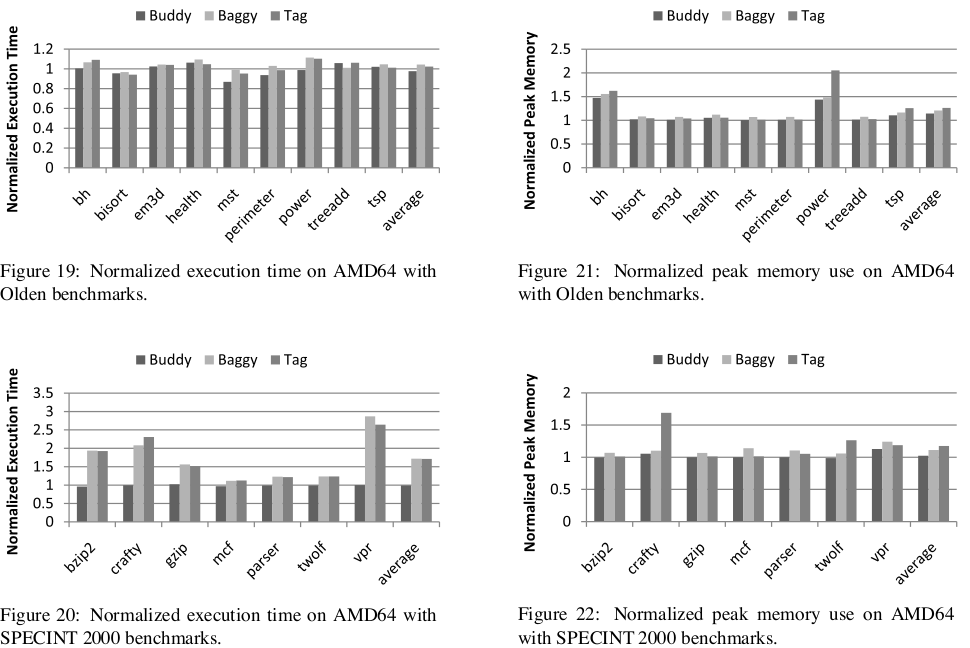
\includegraphics[height=0.8\textheight]{baggy-bounds-perf}
    \end{center}
\end{frame}

\begin{frame}[fragile,label=bbNit]{benign out-of-bounds}
\lstset{language=C,style=small}
    \begin{itemize}
        \item baggy bounds also has support for benign bounds violations:
\begin{lstlisting}
int rawArray[100];
int *array = &rawArray[-1];
// now pretend array's first index is 1
\end{lstlisting}
        \item yes, this is done in real C programs
    \end{itemize}
\end{frame}

\begin{frame}[fragile,label=missingBaggy]{missing from baggy bounds}
    \begin{itemize}
        \item detecting use-after-free bugs
            \begin{itemize}
                \item or other cases of type confusion
            \end{itemize}
        \item detecting errors within an object:
\begin{lstlisting}[language=C,style=small]
struct Foo {
    char buffer[100];
    void (*danger)();
};
\end{lstlisting}
        \item very fancy compiler analyses to eliminate checks
    \end{itemize}
\end{frame}

\begin{frame}{2013 memory safety landscape}
    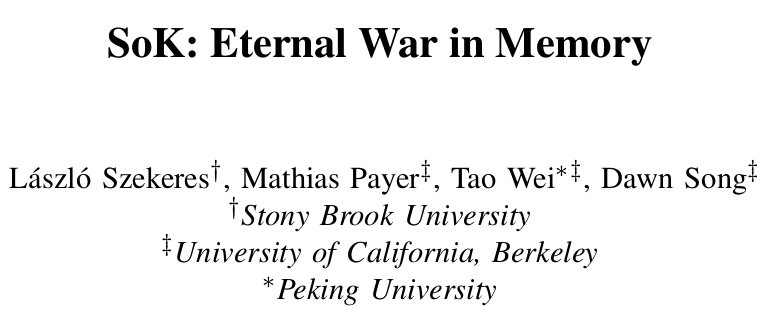
\includegraphics[width=1.0\textwidth]{SoK-eternal-title}
\end{frame}

\begin{frame}{2013 memory safety landscape}
    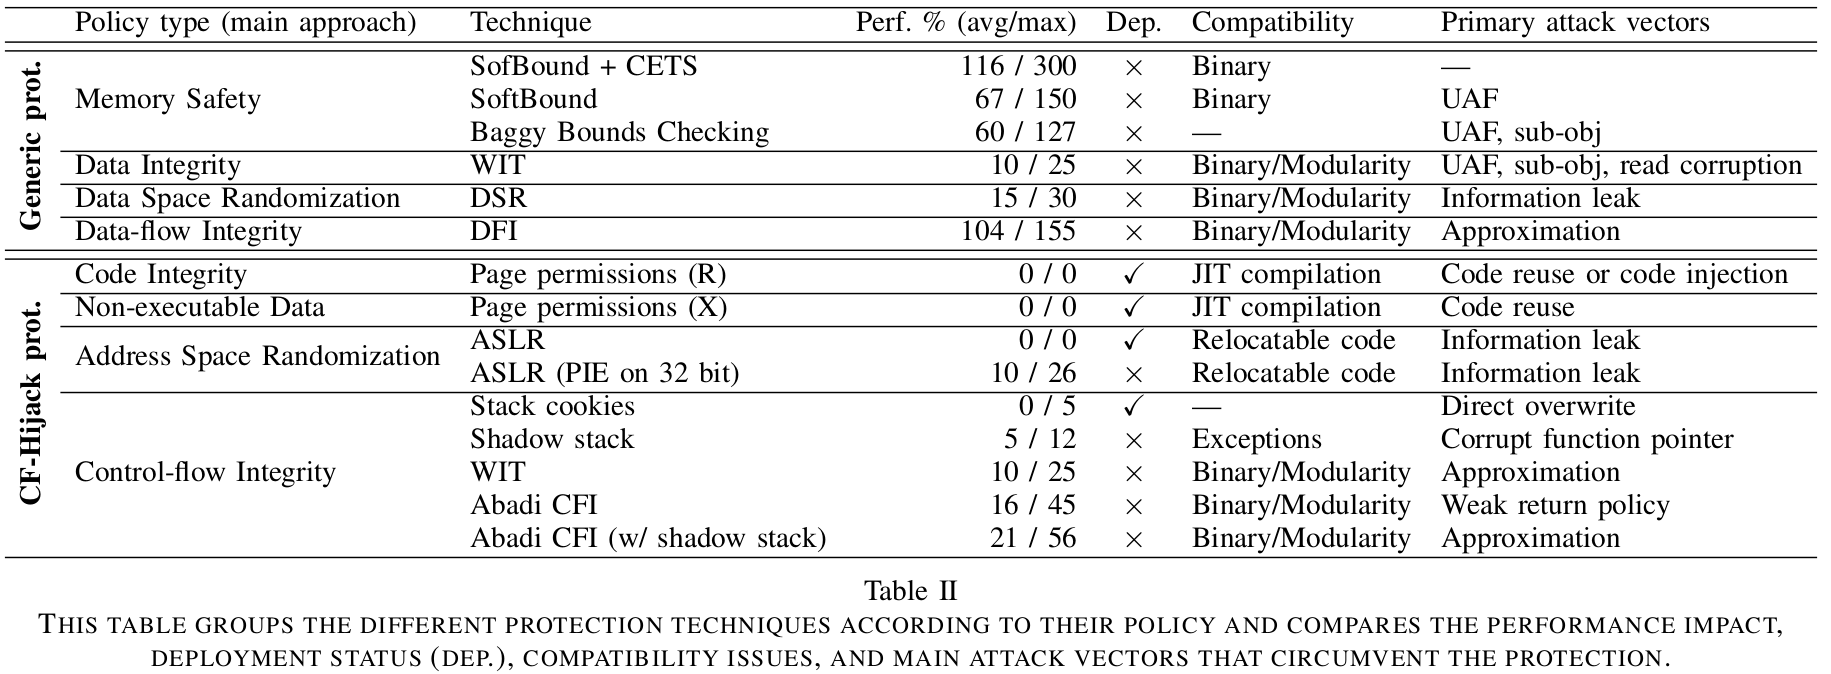
\includegraphics[width=1.05\textwidth]{SoK-table}
\end{frame}

\begin{frame}<1-2>[fragile,label=altTechs]{alternative techniques}
    \begin{itemize}
        \item \myemph<2>{memory error detectors} --- to help with software testing
            \begin{itemize}
            \item reliably detect single-byte overwrites, use-after-free
            \item bitmap for every bit of memory --- should this be accessed
            \item \textbf{not} suitable for stopping exploits
            \item examples: AddressSanitizer, Valgrind MemCheck
            \end{itemize}
        \item \myemph<3>{automatic testing tools} --- run programs to trigger memory bugs
        \item \myemph<4>{static analysis} --- analyze programs and either
            \begin{itemize}
            \item find likely memory bugs, or
            \item prove absence of memory bugs
            \end{itemize}
        \item \myemph<5>{better programming languages}
    \end{itemize}
\end{frame}

\begin{frame}{AddressSanitizer}
    \begin{itemize}
    \item like baggy bounds:
        \begin{itemize}
        \item big lookup table
        \item lookup table set by memory allocations
        \item compiler modification: change stack allocations
        \end{itemize}
    \item unlike baggy bounds:
        \begin{itemize}
        \item check reads/writes (instead of pointer computations)
            \begin{itemize}
            \item only detect errors that read/write \myemph{between objects}
            \item deliberate padding added to detect errors
            \end{itemize}
        \item no power-of-two restriction
        \item table has info for every single byte (more precise)
        \end{itemize}
    \end{itemize}
\end{frame}

\begin{frame}{Valgrind Memcheck}
    \begin{itemize}
    \item similar to AddressSanitizer --- but no compiler modificaitons
    \item instead: is a virtual machine
    \vspace{.5cm}
    \item can't reliably detect stack errors
    \item but works on \myemph{unmodified} binaries
    \end{itemize}
\end{frame}

\againframe<3>{altTechs}

\begin{frame}{automatic testing tools}
    \begin{itemize}
        \item basic idea: generate lots of random tests --- ``\myemph{fuzzing}''
        \item look for segfaults and/or run with memory error detector
        \vspace{.5cm}
        \item blackbox:
            \begin{itemize}
            \item just try random testing
            \end{itemize}
        \item whitebox:
            \begin{itemize}
            \item generate tests by looking at what program does internally
            \end{itemize}
    \end{itemize}
\end{frame}

\againframe<4>{altTechs}

\begin{frame}{static analysis}
    \begin{itemize}
        \item analyze program code directly
        \item some overlap with whitebox testing
        \item complete versus sound
            \begin{itemize}
                \item complete: no false positive
                    \begin{itemize}
                        \item says memory error --- actually a memory error
                    \end{itemize}
                \item sound: no false negative
                    \begin{itemize}
                        \item says no memory error --- actually no memory errors
                    \end{itemize}
            \end{itemize}
        \item many real analyzers \myemph{neither complete nor sound}
        \item sometimes assisted by programmer annotations
            \begin{itemize}
                \item e.g. ``this pointer should not be null''
            \end{itemize}
    \end{itemize}
\end{frame}

\againframe<5>{altTechs}

\begin{frame}{better programming languages}
    \begin{itemize}
        \item get better information from programmer
        \item ideal: eliminate memory errors \myemph{without making program slower}
        \item some overlap with static analysis
            \begin{itemize}
                \item information used to prove no memory errors
            \end{itemize}
        \item example: ``smart pointer'' libraries for C++
        \item example: Rust
    \end{itemize}
\end{frame}

\begin{frame}{other kinds of bugs?}
    \begin{itemize}
        \item many of these techniques work for other security bugs
        \item testing, static analysis, programming language improvements
        \item same basic ideas also applicable
    \end{itemize}
\end{frame}

\begin{frame}{plans for the future}
    \begin{itemize}
        \item assignment using a ``fuzzing'' tool
        \item would like to go over some additional topics:
            \begin{itemize}
            \item command injection bugs
            \item web browser security
            \item whitebox fuzzing (`informed' random testing)
            \item better programming languages --- Rust
            \end{itemize}
        \item I am flexible --- different topics you want?
            \begin{itemize}
            \item sandboxing (another mitigation)
            \item synchornization-related security bugs
            \item static analysis?
            \item new mitigations proposed in research?
            \item other?
            \end{itemize}
    \end{itemize}
\end{frame}
